
%(BEGIN_QUESTION)
% Copyright 2010, Tony R. Kuphaldt, released under the Creative Commons Attribution License (v 1.0)
% This means you may do almost anything with this work of mine, so long as you give me proper credit

Suppose we have an Allen-Bradley model ``SLC 500'' PLC connected to a pair of momentary-contact pushbutton switches and light bulbs as shown in this illustration:

$$\includegraphics[width=15.5cm]{i03760x01.eps}$$

Examine the following relay ladder logic (RLL) program for this Allen-Bradley PLC, determining the statuses of the two lamps provided switch A is pressed by a human operator and switch B is unpressed:

$$\includegraphics[width=15.5cm]{i03760x02.eps}$$

\vskip 20pt \vbox{\hrule \hbox{\strut \vrule{} {\bf Suggestions for Socratic discussion} \vrule} \hrule}

\begin{itemize}
\item{} Identify which LED indicators on the I/O cards' faces would be lit in this condition.
\item{} Describe how this system would respond if a technician used the {\it force} utility to force bit {\tt O:3/4} to a ``1'' state in the PLC's memory.
\end{itemize}

\underbar{file i03760}
%(END_QUESTION)





%(BEGIN_ANSWER)

Output {\tt O:3/4} will activate to energize lamp Y, but the other output (and lamp) will remain off:

$$\includegraphics[width=15.5cm]{i03760x03.eps}$$

%(END_ANSWER)





%(BEGIN_NOTES)


%INDEX% PLC, relating I/O status to virtual elements

%(END_NOTES)


